\chapter{С чего всё началось?}
\section{Что такое фракталы?}
\subsection{Определение фрактала и небольшое пояснение}
Фрактал (лат. fractus — дроблёный, сломанный, разбитый) — множество, обладающее свойством самоподобия (объект, в точности или приближённо совпадающий с частью себя самого, то есть целое имеет ту же форму, что и одна или более частей). В математике под фракталами понимают множества точек в евклидовом пространстве, имеющие дробную метрическую размерность (в смысле Минковского или Хаусдорфа), либо метрическую размерность, отличную от топологической, поэтому их следует отличать от прочих геометрических фигур, ограниченных конечным числом звеньев. Самоподобные фигуры, повторяющиеся конечное число раз, называются предфракталами. 

Т.е фракталом можно называть структуру, состоящую из частей подобных целому.

\subsection{Почему же квадраты это не фракталы?}
Очень хороший вопрос. Если взять кусочек квадрата, то он и будет являться квадратом. Тогда почему же квадрат это не фрактал?
Две вещи, которые не дают квадратам преисполнится до фракталов:
\begin{itemize}
	\item Дробность, изрезанность, о которой мы говорили выше.
	\item Дробная размерность.
\end{itemize}

Секундочку, какая дробная размерность? В школе учили что размерность пространства всегда натуральное число и 0, если геометрический объект наших экспериментов точка. Так мог подумать наш дорогой читатель, давайте разбираться в чем же дело.

Вспомнив школьное определение размерности фигуры, все встает на места:
Если фигуру можно составить из некоторых примитивов, размерность которых мы знаем заранее, то их размерности совпадают. Например:
\begin{itemize}
	\item Точку можно составить только из точки. Размерность 0.
	\item Отрезок можно составить только из отрезков. Размерность 1.
	\item Квадрат можно составить только из квадратов. Размерность 2. И тд.
\end{itemize}

Но если мы попробуем сделать с фракталом на обложке [рис. 1]

\begin{figure}
	\centering
	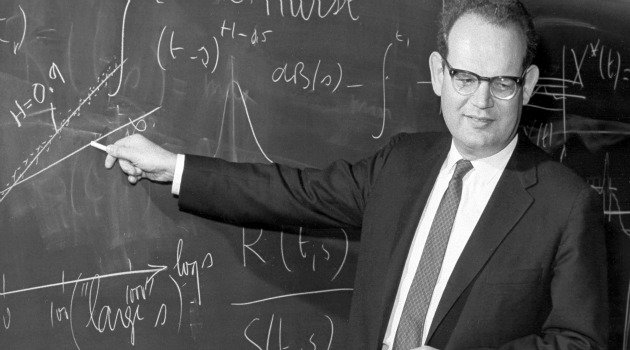
\includegraphics[width=\textwidth]{Benoit-Mandelbrot}
	\caption[рис.1]{Бенуа Мандельброт на одной из своих лекций}
\end{figure}


